\documentclass{article}
\usepackage{hyperref}
\usepackage{amsmath}
\usepackage{amssymb}
\usepackage{pgfplots}
\usepackage{float}
\usepackage{todonotes}
\usepackage{tikz}
\usepackage[shortlabels]{enumitem}

\renewcommand{\Re}{\mathbb{R}}
\newcommand{\Li}{\mathcal{L}}
\newcommand{\Ex}{\mathbb{E}}
\renewcommand{\Pr}{\mathbb{P}}
\newcommand{\Hy}{\mathcal{H}}
\newcommand{\sign}{\text{sign}}
\newcommand{\error}{\text{error}}

\newcommand\bigO[1]{
    \ensuremath{\mathcal{O}\left(#1\right)}
    }

\newcommand{\sigmoidPlot}{
    
    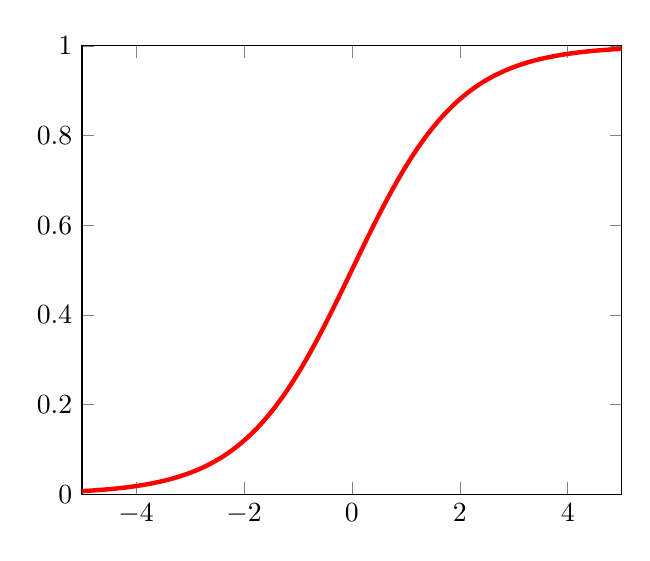
\begin{tikzpicture}
        \begin{axis}[xmin=-5, xmax=5, ymin=0, ymax=1, samples=150]
        \addplot[red, ultra thick] {1/(1+exp(-x))};
        \end{axis}
    \end{tikzpicture}
    
    }

\usetikzlibrary{positioning, calc}
\usetikzlibrary{arrows.meta}

\tikzstyle{circlebox}=[circle,thick,draw=black!75,minimum size=8mm]
\tikzstyle{inputnode}=[circlebox, draw=blue!75]
\tikzstyle{hiddennode}=[circlebox, draw=orange!75]
\tikzstyle{outputnode}=[circlebox, draw=orange!75]
\tikzstyle{simplebox}=[rectangle,thick,draw=black!75,
fill=black!20,minimum size=4mm]
\tikzstyle{textbox}=[rectangle,thick,minimum size=4mm,draw=black!0,
fill=black!0]
\tikzstyle{halfvdistance}=[yshift=-0.7cm]
\tikzstyle{abovebetween}=[xshift=-2.7mm]
\tikzstyle{edgepath} = [-Latex,->,shorten >=1pt,-stealth,semithick, rounded 
corners=5pt]

\def \nodedv {0.735cm}
\def \nodedh {0.65cm}

\tikzset{
    between/.style args={#1 and #2}{
        at = ($(#1)!0.5!(#2)$)
    }
}

\begin{document}
    \section{Subjects}
    \begin{itemize}
        \item What is RNA $2^{nd}$ structure?
        \item Computing a pseudo-knot free RNA $2^{nd}$ structure.
    \end{itemize}
    
    \section{Notes}
    
    \subsection{RNA and second structure}
    Messenger RNA is often described as a linear, unstructured sequence, only 
    interesting for the protein amino acid sequence that it encodes.
    
    However, many non-coding RNA's exist which adopt sophisticated 
    three-dimensional structures, and even catalyse biochemical reactions.  RNA 
    is typically produced as a single stranded molecule, which then folds to 
    form a number of short base-paired stem, this is what we call the seconday 
    structure of the RNA. 
    
    RNA is a polymer of four different nucleotide subunits, we abbreviate them 
    $A,C,G$ and $U$. In DNA, thymine $T$ replaces uracil $U$. $G-C$ and $A-U$ 
    form hydrogen bonded base pairs. $G-C$ form three hydrogen bonds and tend 
    to be more stable than $A-U$ pairs which form only two. Some non-canonical 
    pairs also forms, like the $G-U$ pair, and others which distort regular 
    A-form RNA helices.
    
    Base pairs are approximately coplanar and are almost always 
    \textit{stacked} onto other base pairs. Such contiguous stacked base pairs 
    are called \textit{stems}. In three dimensional space, the stems generally 
    form a regula (A-form) double helix. We typically represent the RNA 
    $2^{nd}$ structure in two-dimensional pictures.
    \\
    \\
    Single stranded subsequences bounded by base pairs are called loops. A loop 
    at the end of a stem is called a \textit{hairpin loop}. Simple 
    substructures which just consist of a stem and a loop is called 
    \textit{stem loops} or \textit{hairpins}. Single stranded bases occuring 
    within a stem are culled a \textit{bulge} or \textit{bulge loop} if the 
    single stranded bases on only on side of the stem. it's called an 
    \textit{interior loop} if there is a bulge on both sides. If a loop 
    connects three or more stems, then it is called a \textit{multibranched 
    loop}.

    Base pairs almost always occur in a nested fashion in RNA secondary 
    structure. Base pairs are nested if we can draw arcs over them, and none of 
    the arcs intersect. Formally, if $i,j$ is a base pair and $i',j'$ is a base 
    pair then $i<i'<j'<j$. If it happens that these arcs would cross, then they 
    are called \textit{pseudo-knots}.
    
    Just to spell it out, this is nexted:
    
    \begin{tikzpicture}
        \node[smallcirclebox] (x1) {};
        \node[smallcirclebox, right =of x1] (x2) {};
        \node[smallcirclebox, right =of x2] (x3) {};
        \node[smallcirclebox, right =of x3] (x4) {};
        
        \path[edgepath]
            (x1) edge [bend left,-] node {} (x4)
            (x2) edge [bend left,-] node {} (x3);
    \end{tikzpicture}
    
    This is juxtaposed:
    
    \begin{tikzpicture}
        \node[smallcirclebox] (x1) {};
        \node[smallcirclebox, right =of x1] (x2) {};
        \node[smallcirclebox, right =of x2] (x3) {};
        \node[smallcirclebox, right =of x3] (x4) {};
        
        \path[edgepath]
            (x1) edge [bend left,-] node {} (x2)
            (x3) edge [bend left,-] node {} (x4);
    \end{tikzpicture}
    
    This is overlapping (pseudo-knot):
    
    \begin{tikzpicture}
        \node[smallcirclebox] (x1) {};
        \node[smallcirclebox, right =of x1] (x2) {};
        \node[smallcirclebox, right =of x2] (x3) {};
        \node[smallcirclebox, right =of x3] (x4) {};
        
        \path[edgepath]
            (x1) edge [bend left,-] node {} (x3)
            (x2) edge [bend left,-] node {} (x4);
    \end{tikzpicture}
    
    If there are no pseudo-knots, then we can represent it as a planar graph, 
    and in general it is easier to find the compute the secondary structure 
    with the least ``free energy'' without the pseudo-knots. Fortunately, there 
    are very few pseudo-knots compared to the number of base pairs in nested 
    secondary structure, so it is usually acceptable to sacrifice the 
    information in pseudo-knots in return of efficient algorithms.
    
    \subsection{Predicting $2^{nd}$ RNA structure}
    Usually, when we want to predict the secondary stucture, we will try to 
    minimize the amount of ``free energy''. The first example we will look at, 
    bases the prediction on the primary structure (the simple sequence) only. 
    For this we have Nussinov and Zuker's Mfold algorithm. Other methods use 
    comparative structure prediction which is based on a prior alignment. As 
    well as probabilistic methods.
    
    \subsubsection{Nussinov}
    When we need to predict the secondary structure, there are many plausible 
    secondary structures. An RNA of length $200$ has over $10^{50}$ possible 
    base-paired structures. Therefore, we need both a function that assigns the 
    correct structure the highest score, and an algorithm for evaluating the 
    scores.
    
    Nussinov attempts to find the structure with the most base pairs, it is a 
    dynamic programming approach, which calculate the best structure for small 
    subsequences and work outwards. Let's first introduce som notations:
    \begin{itemize}
        \item $seq$ the RNA sequence of $\{A,C,G,U\}$
        \item $seq[i,j]$ the RNA sequence from position $i$ to $j$
        \item $str$ the best $2^{nd}$ structure for $seq$ of $\{(,),.\}$
        \item $str[i,j]$ the best $2^{nd}$ structure for $seq[i,j]$
        \item $score[i,j]$ the number of base pairs in $str[i,j]$
    \end{itemize}
    In the Nussinov algorithm we look at four cases:
    
    $i$ being unpaired and $str[i+1,j]$, that is we just prepend $i$ to the 
    rest of the structure:
    
    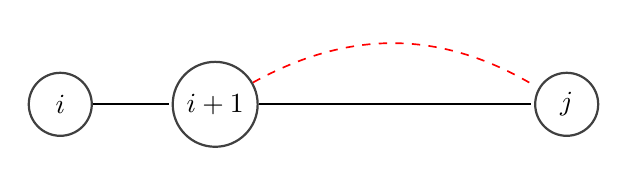
\begin{tikzpicture}
        \node[circlebox] (x1) {$i$};
        \node[circlebox, right =of x1] (x2) {$i+1$};
        \node[right =of x2] (x3) {};
        \node[right =of x3] (x4) {};
        \node[circlebox, right =of x4] (x5) {$j$};
        
        \path[edgepath,red,dashed]
            (x2) edge [bend left,-] node {} (x5);
            
        \path[edgepath,-]
            (x1) edge node {} (x2)
            (x2) edge node {} (x5);
    \end{tikzpicture}
    
    $j$ being unpaired and $str[i,j-1]$, that is we just append $j$ to the rest 
    of the structure:
    
    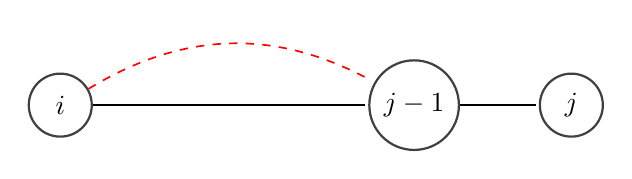
\begin{tikzpicture}
        \node[circlebox] (x1) {$i$};
        \node[right =of x1] (x2) {};
        \node[right =of x2] (x3) {};
        \node[circlebox, right =of x3] (x4) {$j-1$};
        \node[circlebox, right =of x4] (x5) {$j$};
        
        \path[edgepath,red,dashed]
            (x1) edge [bend left,-] node {} (x4);
        
        \path[edgepath,-]
            (x1) edge node {} (x4)
            (x4) edge node {} (x5);
    \end{tikzpicture}
    
    $seq[i] \cdot seq[j]$ and $str[i+1, j-1]$, that is we add the base-pair 
    $i,j$ to the rest of the structure:
    
    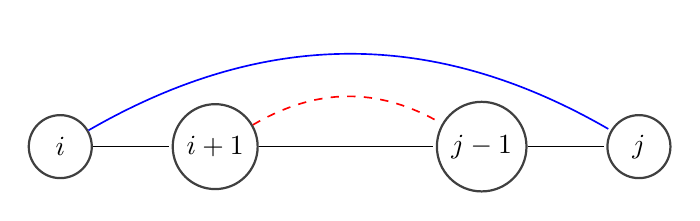
\begin{tikzpicture}
        \node[circlebox] (x1) {$i$};
        \node[circlebox, right =of x1] (x2) {$i+1$};
        \node[right =of x2] (x3) {};
        \node[circlebox, right =of x3] (x4) {$j-1$};
        \node[circlebox, right =of x4] (x5) {$j$};
        
        \path[edgepath,red,dashed]
            (x2) edge [bend left,-] node {} (x4);
            
        \path[edgepath,blue]
            (x1) edge [bend left,-] node {} (x5);
        
        \path[edgepath,-]
            (x1) edge node {} (x2)
            (x2) edge node {} (x4)
            (x4) edge node {} (x5);
    \end{tikzpicture}
    
    $str[i,k]$ and $str[k+1,j]$ for some $i<k<j$, that is we just concatenate 
    the two structures:
    
    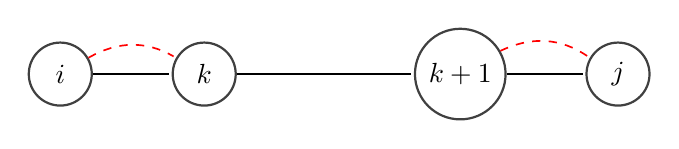
\begin{tikzpicture}
        \node[circlebox] (x1) {$i$};
        \node[circlebox, right =of x1] (x2) {$k$};
        \node[right =of x2] (x3) {};
        \node[circlebox, right =of x3] (x4) {$k+1$};
        \node[circlebox, right =of x4] (x5) {$j$};
        
        \path[edgepath,red,dashed]
            (x1) edge [bend left,-] node {} (x2)
            (x4) edge [bend left,-] node {} (x5);
        
        \path[edgepath,-]
            (x1) edge node {} (x2)
            (x2) edge node {} (x4)
            (x4) edge node {} (x5);
    \end{tikzpicture}
    
    We then find the one of these cases which returns the highest score, which 
    can be described formally as:
    \begin{equation*}
        score[i,j]=\begin{cases}
        0\text{ if }j-1<2\\
        \max\begin{cases}
        score[i+1,j]\\
        score[i, j-1]\\
        score[i+1, j-1]+1 if seq[i]\cdot seq[j]\\
        max_{i<k<j-1}(score[i,k]+score[k+1,j])
        \end{cases}
        \end{cases}
    \end{equation*}
    
    We have to save all the results in table of space \bigO{n^2} and it will 
    take \bigO{n^3} to compute. We then simply start at the top-right corner of 
    the table produced by the algorithm (the index corresponding to the first 
    and last index) and traceback through the table. The path we trace back 
    through the table is the optimal structure.
    
    This can also be described as a stochastic CFG:
    \begin{align*}
        S &\rightarrow aS|cS|gS|uS &\text{($i$ unpaired)}\\
        S &\rightarrow Sa|Sc|Sg|Su &\text{($j$ unparied)}\\
        S &\rightarrow aSu|cSg|gSc|uSa &\text{(i,j pair)}\\
        S &\rightarrow SS &\text{bifurcation}
    \end{align*}
\end{document}